\chapter{Case Context}
Our case is located in Rwanda. Rwanda is on the border of central and east Africa and is located just south of the border of Uganda. The area is $26338km^2$ which makes it $\approx 7\%$ of Norway. Still their population count is over the double that of Norway's. In 2014 the population count in Rwanda was $12337138$ citizens which makes their population density $468.42citizen/km^2$. Compared to Norway with a population density at $13.26$. There are no strict criteria for calling a country a developing one, but if the term is to be used, Rwanda is one of them. \gls{gni} is a way of measure how much value is added by all producers who are resident in a country. The world bank did a \gls{gni} per. capita ranking of the world's countries in 2012 and Rwanda made it at 195th of the 213th economies ranked. The world bank categories economies in four classes:
\begin{description}
\item[\textbf{High Income:}]{$[\$12616, \$\infty]$}
\item[\textbf{Upper Middle Income:}]{$[\$4086, \$12615]$}
\item[\textbf{Lower Middle Income:}]{$[\$1036, \$4085]$}
\item[\textbf{Low Income:}]{$[-\$\infty, \$1035]$}
\end{description}

By this, Rwanda is in the lowest income category with $\$600$ per. citizen, and in this paper, a developing country. It is noteworthy to say that with a population density at $13.26$, Rwanda's population would be $\approx 354509$. Rwanda's \gls{gni} in 2012 is $\$6858 \circ 10^{6}$, making their GNI per. citizen $\approx 19345$. This would argue for making more cost effective solutions and lowering the fertility rate in order to have a sustainable economy. 

\cite{rw:snl}
\cite{ssb:folketall}
\cite{gni:wb}
\cite{gni:wbper}

\section{Brief History}
The first inhabitants of Rwanda was probably the ancestors of Twa people. Findings suggesting this goes back to somewhere between 8000\gls{bc}--3000\gls{bc}. Jumping forward to around 700\gls{bc}--\gls{ad}500 there are evidence suggesting that the Bantu people entering Rwanda. The Bantu's was first farmers and then cattle owners. The Hutu's are believed to be mostly farmers and Tutsi cattle owners so it is natural to assume that this is the source for making any difference between the two peoples. There is a Tutsi rule around \gls{ad}1800, but at a conference in 1890 Rwanda was given to Germany. They favored the Tutsi people and contributed to ethnic discrimination. After World War 1, Rwanda was ruled by Belgium. The introduced identity cards that would categorize every individual as a Tutsi, Hutu, Twa or Naturalized. Under Belgium the Tutsi was still favored. In \gls{ad}1959 Hutu activist began killing Tutsi people, making 20000--100000 Tutsi flee the country. In \gls{ad}1962 Grégoire Kayibanda was the first elected president. He sat out to abolish the Hutu suppression, but that led to Tutsi discrimination. In \gls{ad}1973 there was a military coup by president Habyaramana. Up until \gls{ad}1990 there was a pro Hutu discrimination. 
In \gls{ad}1990 the Tutsi dominant \gls{rpf} lead by Paul Kagame (current president of Rwanda) invaded Rwanda from the north. 
This is the start of a civil war lasting up until a peace agreement in 93. In \gls{ad}1994 president Habyaramana's plane is shot down and started the history's most brutal genocide. 800000--1000000 Tutsi killed by Hutu in 3 months. Stopped by \gls{rpf} when they entered Kigali in July the same year. The first president after the genocide was the Hutu president Pasteur Bizimungu, followed by the \gls{rpf} general, Paul Kagame. After the genocide many fled the country. An estimate of 1 million Hutu fled to Zaire, now renamed and known as \gls{drc}. In 1996 Rwanda invaded \gls{drc} and assisted on allocate the president and started the first Congo war. In 1998 they were asked to back out their forces, but Rwanda refused. This was the start of the second Congo war. After peace negotiations the Rwandian forces pulled out of \gls{drc} in 2002.

\section{More Recent}


\cite{rw:snl}
\cite{rw:wiki}
\cite{hutututsi:wiki}

\section{Health Information System Programme}
The \gls{hisp} is a global network established, managed and coordinated by the Department of Informatics at the University of Oslo. They design, implement and sustain Health Information Systems by a participatory approach. This means including the local users when developing the system in hopes of a more sustainable and successful projects. The system developed aims for supporting health care delivery and information flows in selected health facilities, districts and provinces. 

\begin{description}
\item[\textbf{Vision}]To strengthen the development and use of integrated health information systems within a public health inspired framework in India and
the South Asian region.
\item[\textbf{Mission}]To enable networks of collaborative action with like-minded actors
who aspire to the ideology of open source software, open standards
and decentralized decision-making to create complementary strengths
in providing integrated and public health friendly health information
systems.
\end{description}

In the 1970 and 80's the HISP approach to action research and system design was influenced by a number of union based action research projects in Scandinavia. The focus were on empowering workers who were affected or threatened by new technology. Methods may have changed over time, but the philosophy remains the same. Explore ways in which disadvantaged people could appropriate \gls{ict}'s for their own empowerment. Original key member of the HISP team had background as social political activists in the anti apartheid struggle and other social movements. DHIS, a software organized and developed within the HISP network, was actually born out of the political processes  following the fall of apartheid. During apartheid and until 1994 there were 14 departments of health in South Africa. Because of this fragmentation it was a lot of different procedures, collection tools and data definitions.

\cite{hisp:uio}
\cite{historyhisp:uio}
\cite{abouthisp:india}

\subsection{HISP Strategy}
The core focus of \gls{hisp} is \gls{dhis2}. It through this software that \gls{hisp} will effectively make changes. \gls{dhis2} are now active in 46 countries around the world. This includes 70\% of the global fund high impact countries and 55\% of the \gls{coia} countries.
\gls{hisp} are based at the \gls{uio}. This is were the core developers of \gls{dhis2} are located. 

\begin{figure}
\centering
<<<<<<< HEAD
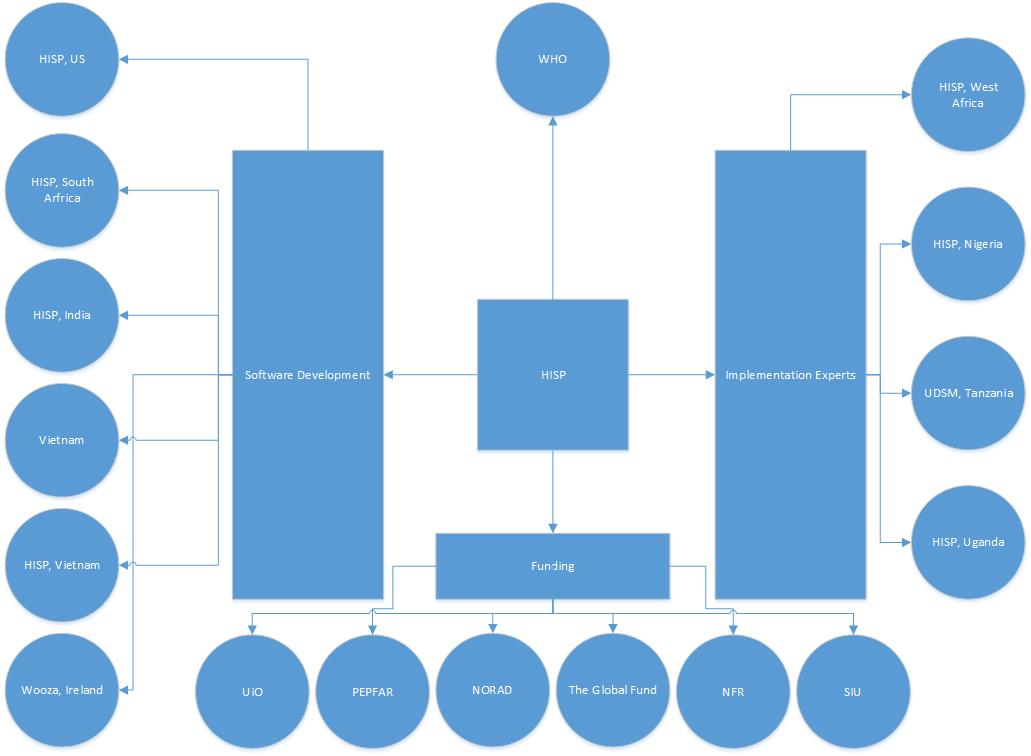
\includegraphics[width=\textwidth]{context/img/networkOfAction}
=======
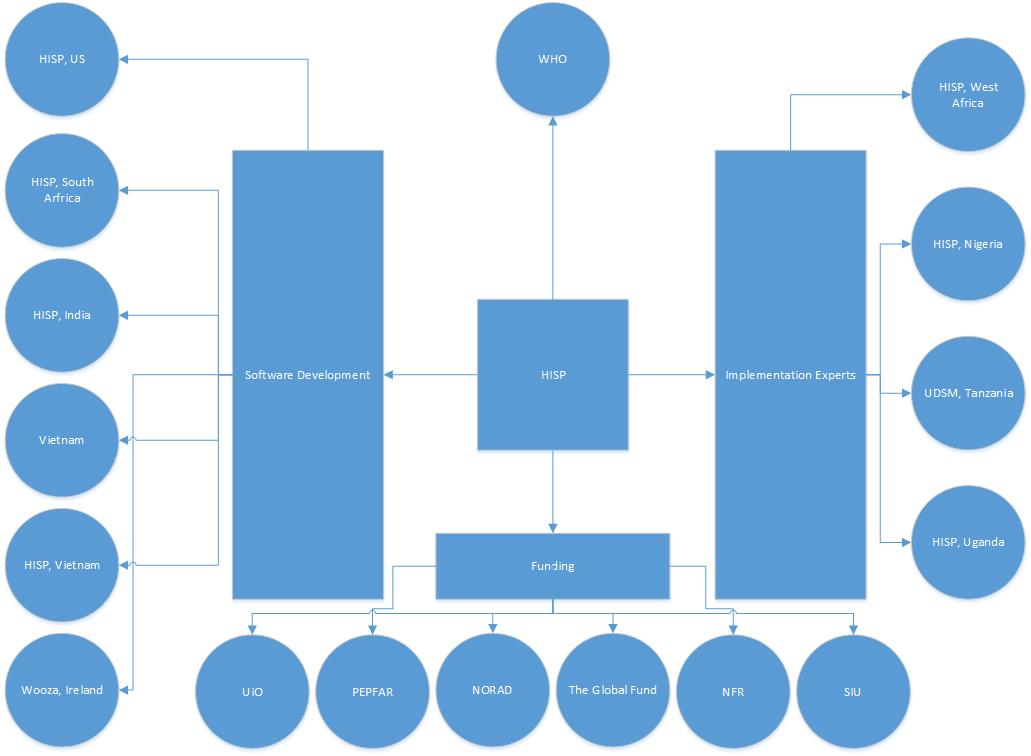
\includegraphics[width=\columnwidth]{context/img/networkOfAction}
>>>>>>> 67309e5eaf802120ae711c557522bece188d36aa
\caption{HISP Network of Action}
\label{fig:hispnet}
\end{figure}

One of \gls{hisp}'s biggest strengths is in their network of action. As illustrated in figure \ref{fig:hispnet}. There is a huge support network for facilitating the development and implementation of \gls{dhis2} and is clearly one of the key success factors of why \gls{dhis2} has been so successful in strengthening the health infrastructure world wide. Recently \gls{hisp} is trying to add to network the East-Africa region. \gls{hisp} East-Africa will include countries like Tanzania, Rwanda, Uganda and Kenya. Making relations between countries is essential for sustainability purposes. Sharing experiences and knowledge through neighboring countries is beneficial for sorting out local implementation problems. \gls{hisp} has been able to arrange for these network building activities with \gls{dhis2} workshops and academies. The primary focus is to train users in the use and implementation of \gls{dhis2}, but a beneficial side effect is network building cross countries. 
With \gls{dhis2} there has been great progress with the process of gathering of data, but two issues remain. Data quality and using data for action. These to areas are now focus areas for the \gls{hisp}-team at \gls{uio}.

\cite{strategyhisp:uio}
\cite{networkhisp:uio}
\cite{jbemss:noa}

\section{District Health Information System}
\begin{figure}
\centering
<<<<<<< HEAD
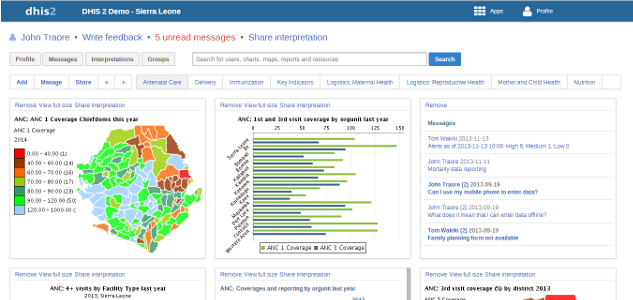
\includegraphics[width=\textwidth]{context/img/dhis2Dash}
=======
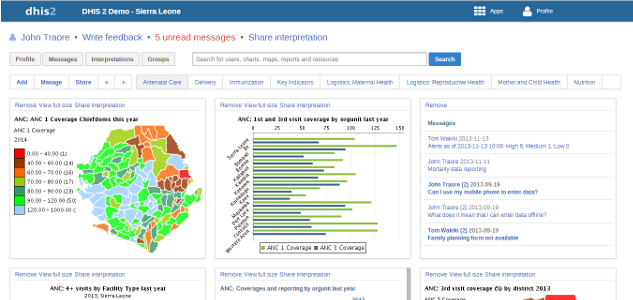
\includegraphics[width=\columnwidth]{context/img/dhis2Dash}
>>>>>>> 67309e5eaf802120ae711c557522bece188d36aa
\caption{Screenshot of Dashboard}
\label{fig:dash}
\end{figure}
\gls{hisp}'s main product is \gls{dhis2}. In short, it is an open source software to manage health information data. It also facilitates both the gathering and presentation of the data. With the aid of this program we are able to collect data on site independent of location and to present those data on the same terms. Usually dependent on an internet connection, but it is possible to gather data on a regular \gls{gsm} network. The importance of this last quality is \textit{huge} in underdeveloped countries. Internet is nowadays usually taken for granted in most places, but when it comes to villages located outside internet coverage, even a mobile connection cannot be taken for granted. In 2012 there was an internet coverage of $33.4\%$ of the worlds population, so assuming an internet connection when working on a global scale is unwise. The system manages data as predefined variables called data elements. These are then grouped together with formulas and description in order to adapt to a health environment. This feature makes it very adaptable to different use cases. We see new systems almost daily nowadays. The smart phone era as boomed the software development, so the need for interoperability is ever increasing. Because of this, a system must be able to work as a piece of the puzzle rather than a silo, but then again new challenges arises. Standardization across departments and health instances needs to be made and it calls for an increased level of cooperation and transparency.

\subsection{Gathering}
\gls{dhis2} allows for data entry for as low-tech as \gls{sms} to the new high-tech smart phones. As mentioned earlier, \gls{sms} support is very important since over half of our population does not have internet coverage. 

\begin{table}
\centering
\begin{tabular}{|l|l|}
\hline
Phone Number: & 2000 \\
\hline
Message: & Stock condom11 \\
\hline
\multicolumn{2}{|c|}{\fbox{Send}} \\
\hline
\end{tabular}
\caption{Example SMS}
\label{table:examplesms}
\end{table}

An example \gls{sms} in table \ref{table:examplesms}. One use case is that a \gls{chw} would like to report the stock on condoms at the end of month. The user would usually go through the following steps.
\begin{enumerate}
\item Enter the phone number assigned the reporting service.
\item Enter the codeword for this type of report.
\item Enter the codeword for the item that is being reported followed by a integer value.
\item Hit send.
\end{enumerate}
There are some extra features, but this is the basic idea. At a first glance, this seem alright, but in most cases there are more than one item involved. Let's say that our example message could represent an average reported \gls{sms} and that the standard \gls{sms} is restricted to be 160 characters long. The codeword is 5 chars. The codeword for the item is 6 and the value is 2. One would usually like to have some kind of separator for each item, so we +1 here. That makes room for approximately 17 items pr. message. I don't know about the general population, but I know it is a pain to write 160 char \gls{sms}'s on a button based phone and if you have more than 17 items one has also to write another \gls{sms}. Also, it is very easy to make mistypes. So it is preferable to report using some of the more advanced devices. But, better than not being able to report. A little more sophisticated option is using a simple phone. These are still cheaper than the most basic smart phones and widely used in underdeveloped countries. They offer a basic \gls{gui} that offers some more description than the cryptic codes. A note on the \gls{sms} entry is that it is usually supplemented with a reporting card that describes the different codes. The more high-tech devices has support for modern browsers so data entry would be very similar to a any other \gls{html} form. 

\begin{figure}
\centering
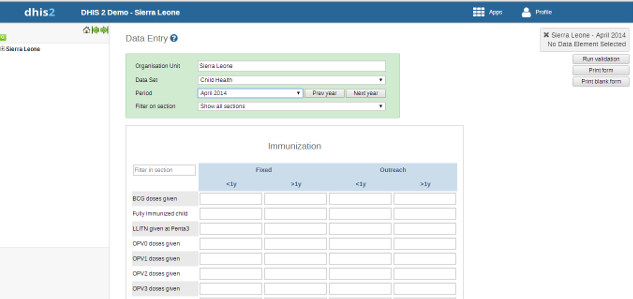
\includegraphics[width=\columnwidth]{context/img/dhis2DataEntry}
\caption{Screenshot of data entry in regular browser.}
\label{fig:dataentry}
\end{figure}

\subsection{Managing}
\begin{figure}
\centering
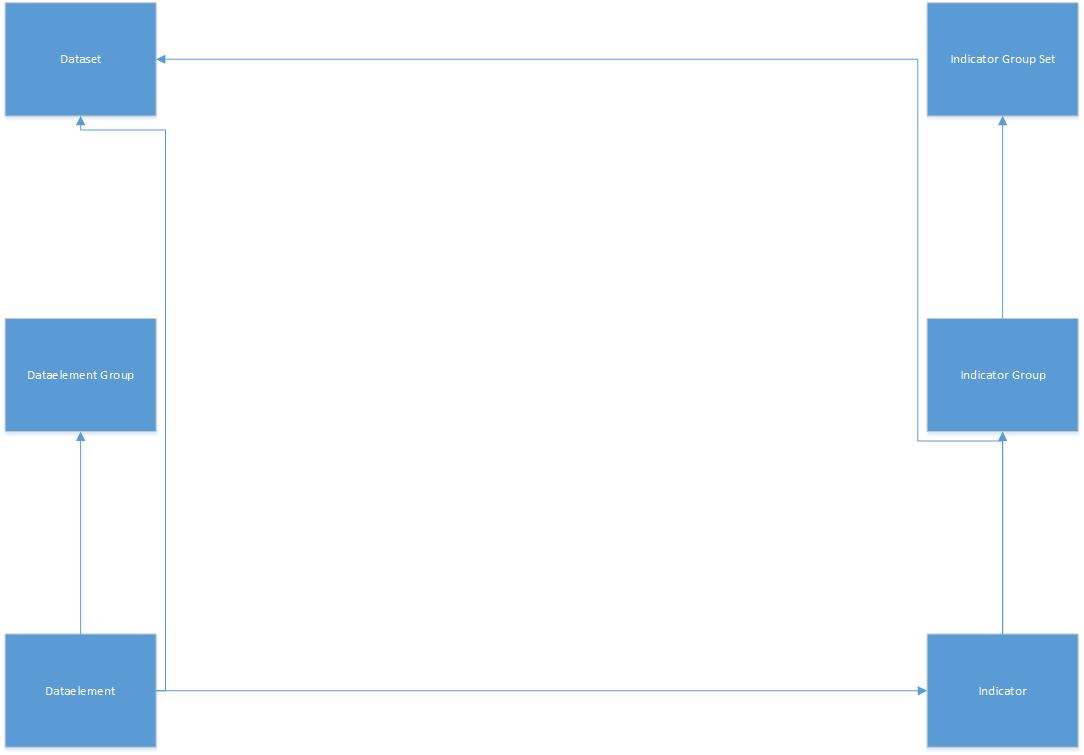
\includegraphics[width=\columnwidth]{context/img/dataStructure}
\caption{Basic Data Structure}
\label{fig:structure}
\end{figure}
Once the data are inside the system it is managed with a data structure designed specifically for \gls{dhis2}, see figure \ref{fig:structure}. At the bottom of the hierarchy and the most basic structure is the dataelement. It is essentially a value of a certain type. Any variable value in the system would usually be a dataelement. The dataelement also has several attributes like a datestamp, description etc. Now, with these elements, one can either combine several or make some mathematical manipulations to them. This variable are then stored indicators. Both of these data types can be grouped together in groups as dataelement group or indicator group. The indicator group can further be classified in indicator group set. This then a group of groups. The most frequently used group type is the data set. It can be a combination of dataelements and indicators. 
All of these data structure comes with descriptions and other kind of meta data in order to be able to analyze the data in an efficient manner.


\subsection{Presenting}
\begin{figure}
\centering
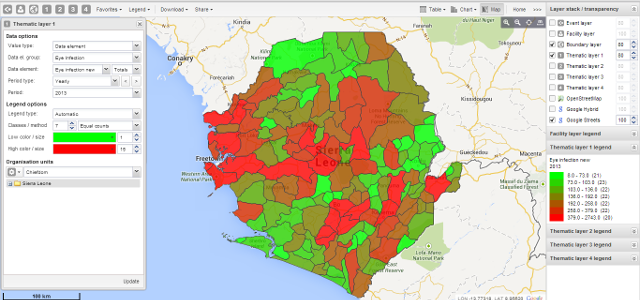
\includegraphics[width=\columnwidth]{context/img/gisExample}
\caption{GIS Example}
\label{fig:gis}
\end{figure}
There are several ways of looking at data in \gls{dhis2}. Of them the most interesting is the \gls{gis}, as seen in figure \ref{fig:gis}. In the figure one can see a count of eye infection in 2013 based on color and Chiefdoms. Green being low and red high. There is a sense of overview by looking at this kind of map. While getting a graphical visualization one has numbers pinpointing the exact number range. Extremely useful when in need to get an updated status on a situation. Some other tools for analyzing and visualizing data is the pivot table, the basic charts and the generation of reports.

\subsection{Application Development}
\gls{dhis2} is meant to be a platform for health information. As a result from silos forming in different departments of the health sector, the choice of health information systems are different. This causes a fragmentation that makes interoperability between systems hard to achieve. As a response to this problem, \gls{dhis2} is now being designed to work much like an appstore. This allows users to develop their own applications that meets their specific needs while keeping the core functionality of \gls{dhis2}. Not only does this benefit the users, but makes collaboration between developers much easier. 


\begin{table}
\centering
\begin{tabular}{|p{4cm}|p{4cm}|p{4cm}|}
\hline
\textbf{Complete national implementation} & \textbf{Adoption by programs or partial national roll-out} & \textbf{Pilot stage or early phase in roll-out} \\
\hline
Bangladesh & Colombia & Afghanistan\\
Ghana & Laos & Algeria\\
India & Malawi & Benin\\
Kenya & Mozambique & Bhutan\\
Liberia & Nigeria & Burkina Faso\\
Rwanda & Sierra Leone & Cameroon\\
Tanzania & Solomon Islands & Congo Brazzaville\\
The Gambia & South Africa & Cote d'Ivoire\\
Uganda & Tajikistan & \gls{drc}\\
Zambia & Vietnam & Guinea Bissau\\
Zanzibar & Zimbabwe & Iraq\\
 & & Mexico\\
 & & Myanmar\\
 & & Namibia\\
 & & Nepal\\
 & & Niger\\
 & & North Korea\\
 & & Samoa\\
 & & Senegal\\
 & & South Sudan\\
 & & Sudan\\
 & & Timor Leste\\
 & & Togo\\
 & & Vanuatu\\
\hline
\end{tabular}
\caption{Countries using DHIS2}
\label{table:countriesusing}
\end{table}

\begin{figure}
\centering
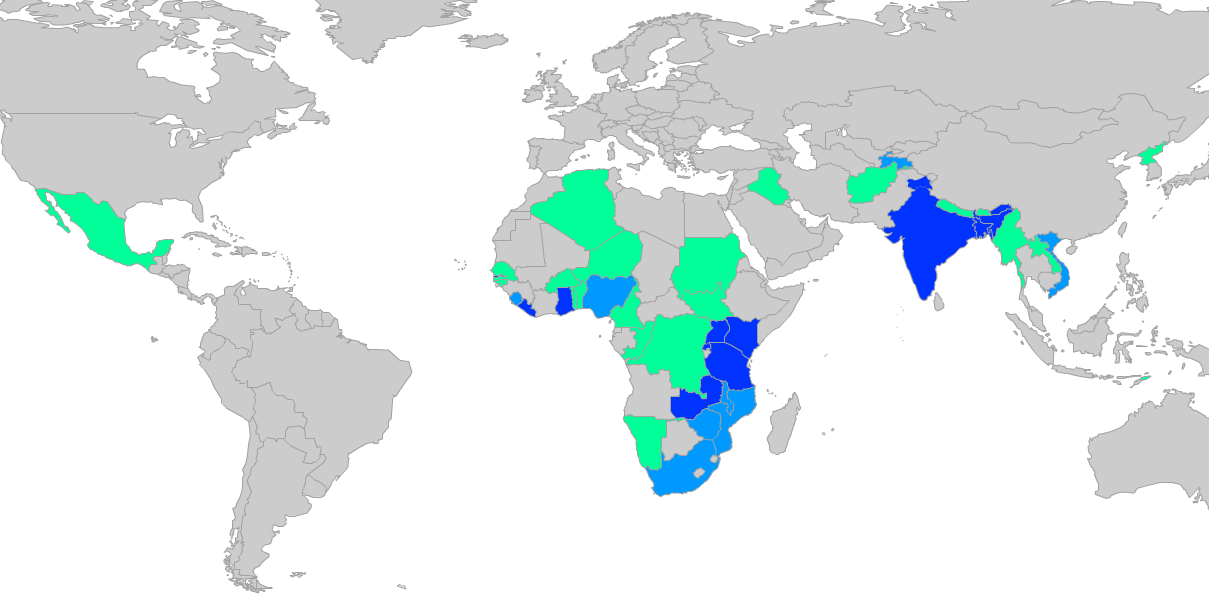
\includegraphics[width=\columnwidth]{context/img/countriesUsing}
\caption{(Blue, National rollout)-(Light-Blue, Programs/partial)-(Green, Pilot/early phase)}
\label{fig:countriesusing}
\end{figure}


\cite{countries:dhis2org}
\cite{internet:stats}

\begin{figure}
\centering
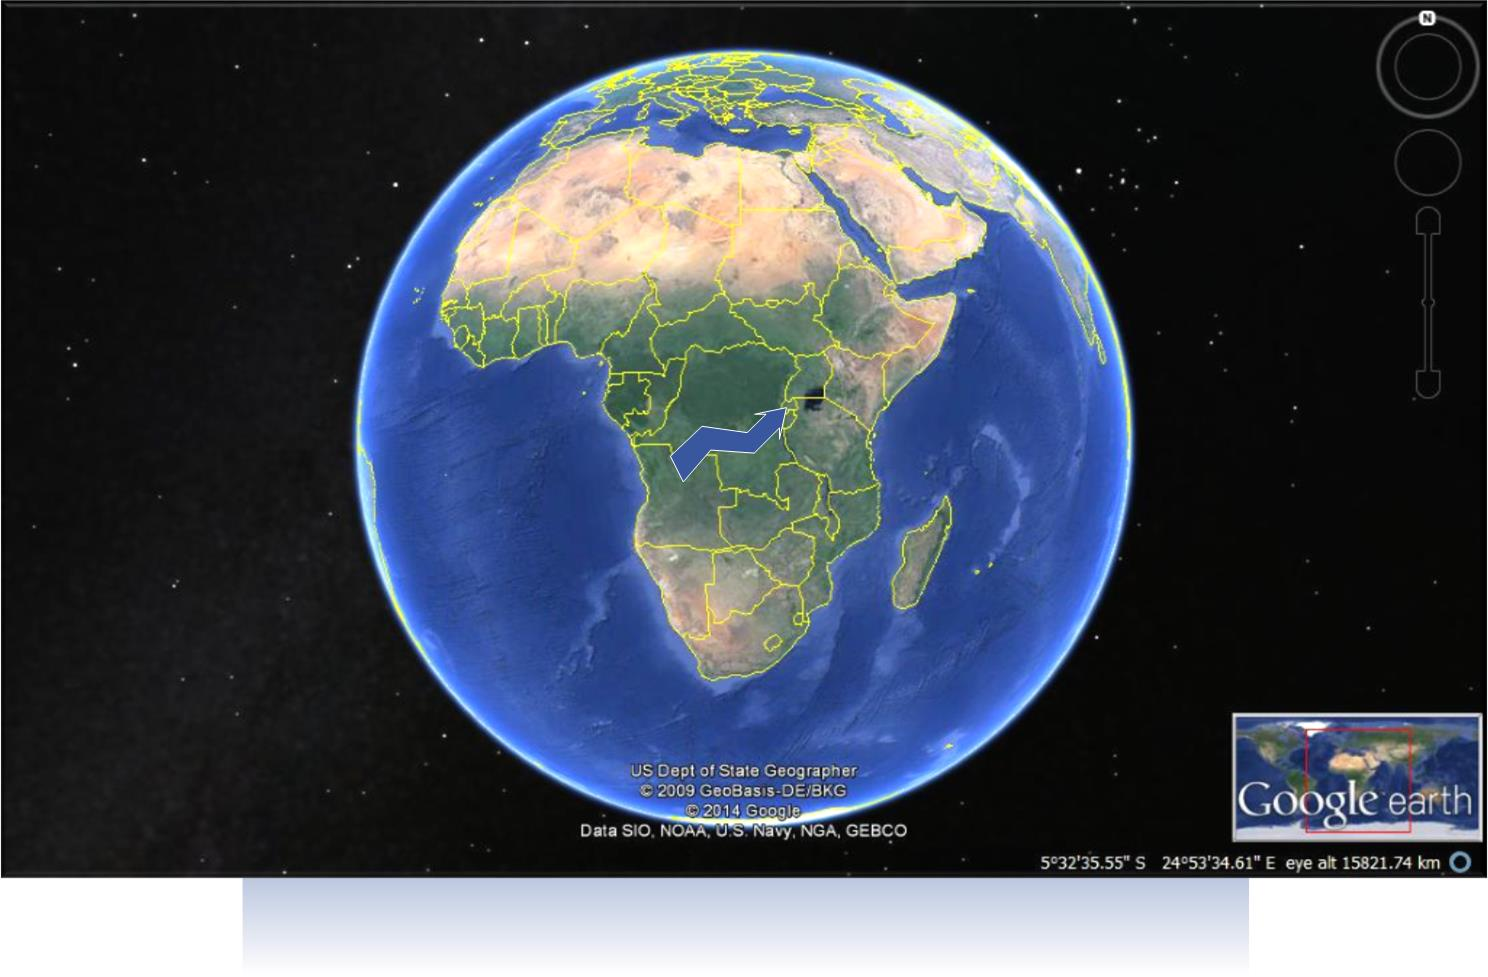
\includegraphics[width=\columnwidth]{context/img/africa}
\label{fig:africa}
\caption{Africa}
\end{figure}

\begin{figure}
\centering
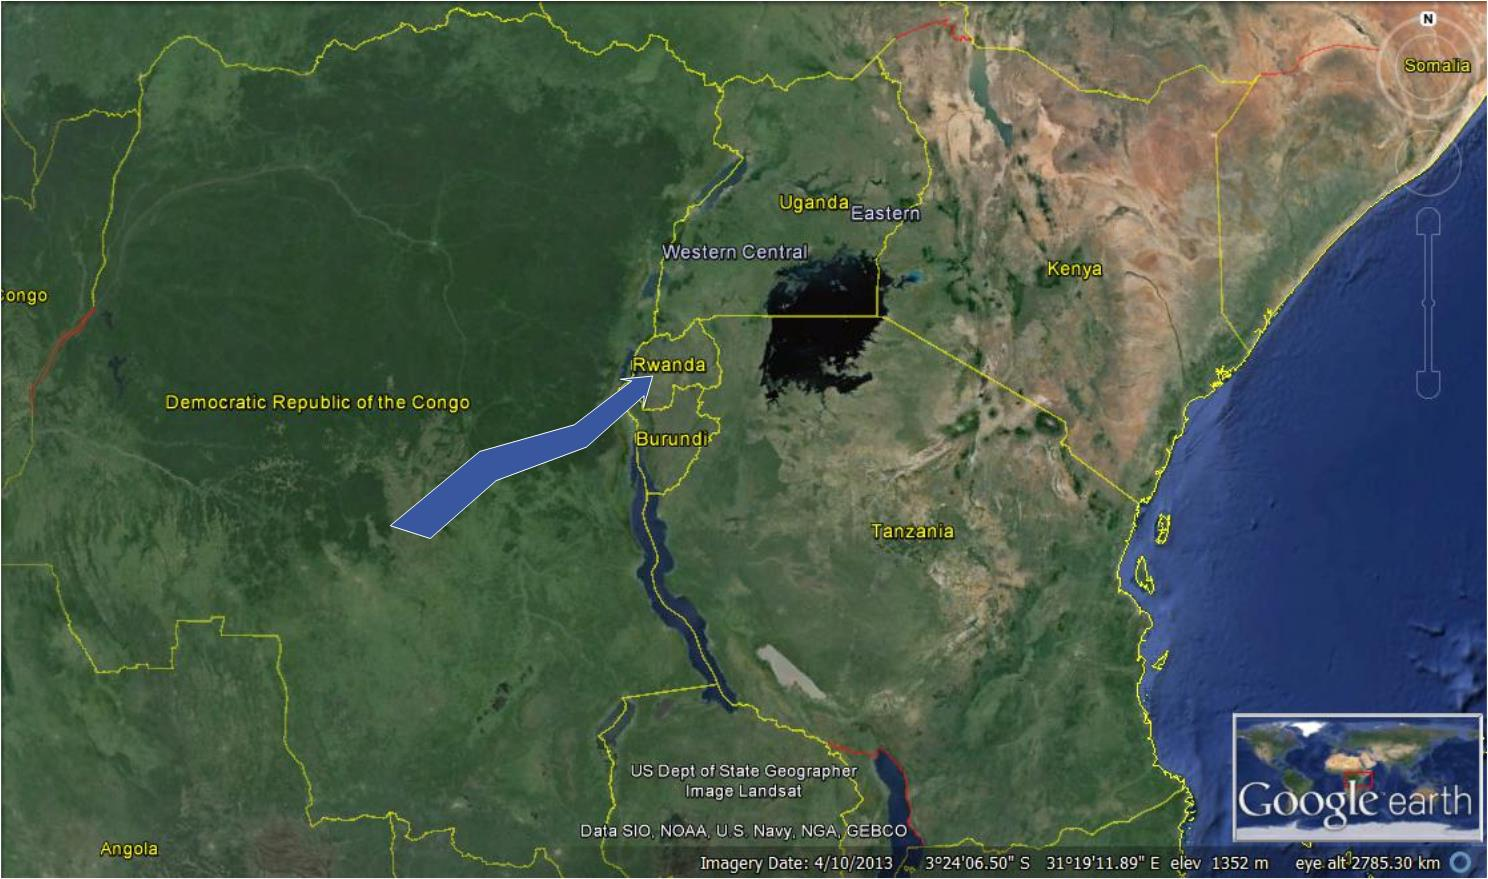
\includegraphics[width=\columnwidth]{context/img/eastAfrica}
\label{fig:east_africa}
\caption{East Africa}
\end{figure}

\begin{figure}
\centering
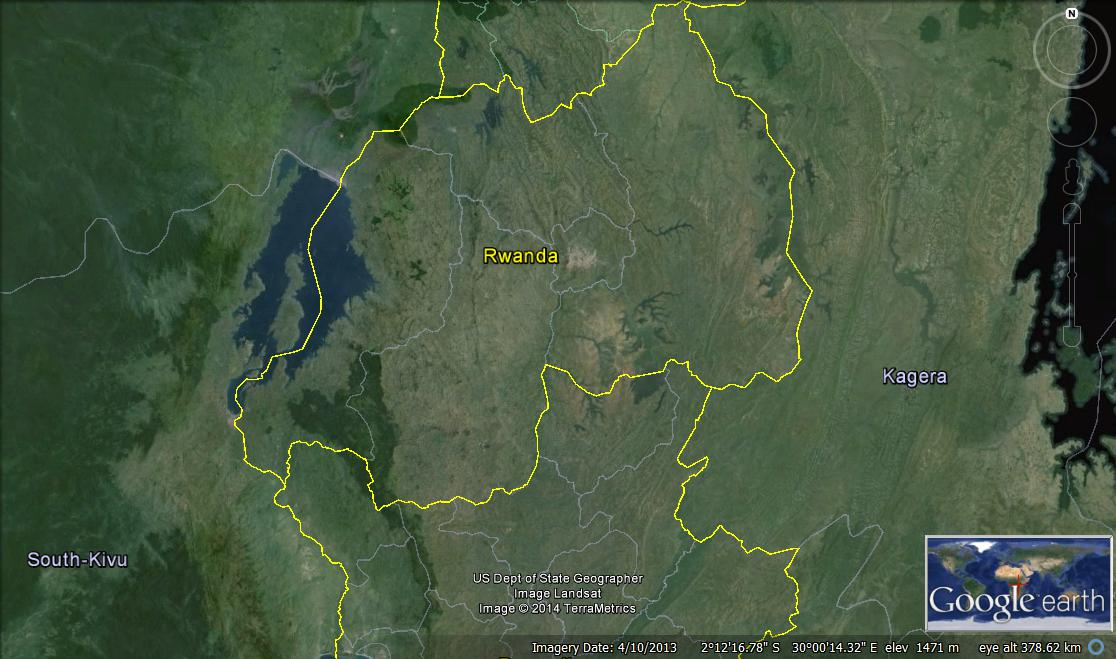
\includegraphics[width=\columnwidth]{context/img/rwanda}
\label{fig:rwanda}
\caption{Rwanda}
\end{figure}

\section{Administrative Structure}
Rwanda has a strict hierarchical structure in their country. The country is divided in Provinces, Districts, Sectors, Cells and Villages.

\begin{figure}
\centering
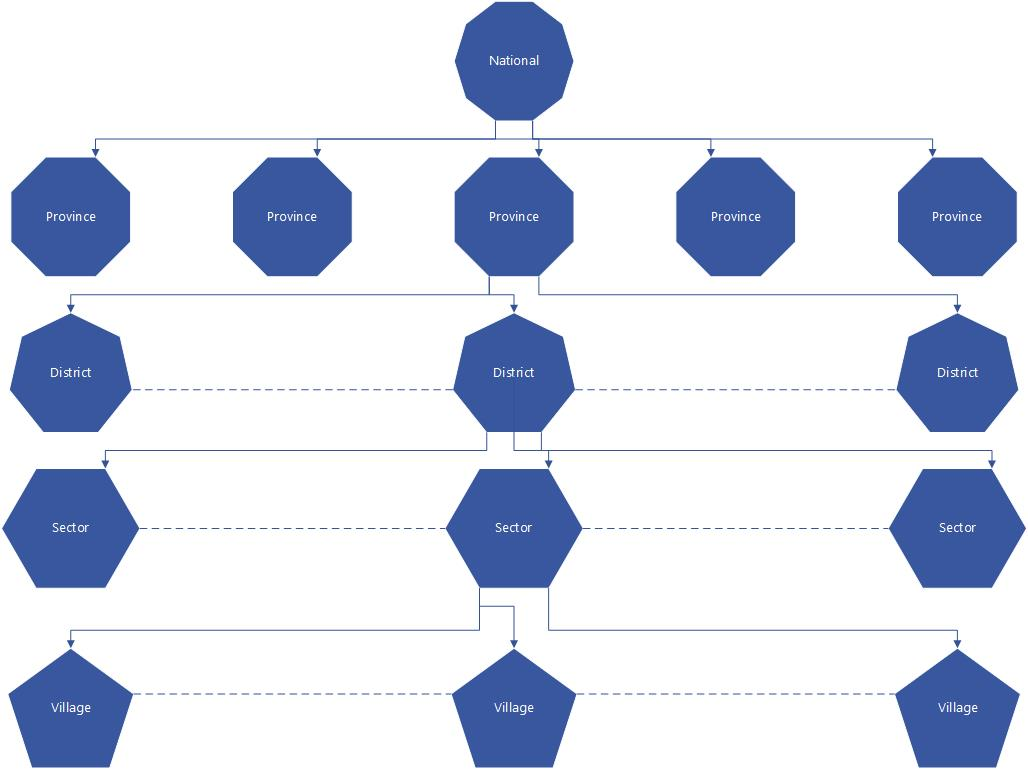
\includegraphics[height=10cm]{context/img/rwandaAdminStructure}
\label{rwanda_admin_structure}
\caption{Rwandas Administrative Structure}
\end{figure}

The level closest to the people is the Village. Here problems, priorities and needs of the people at a grass root level are identified and addressed. Above is the Cell level. Cells are managed by technicians and and a political team. Technical and key political matters are managed here. Further up in the hierarchy is the Sector level. The people participate here through their elected representatives. Sectors are collected in Districts which are the basic political-administrative unit in the country. Just under the national level the country is divided into five provinces. These serves mainly as advisor to the decentralized entities and coordinates development activities. \cite{mlg:admin}

This division is used to make areas more multi-ethnic and to decentralize power as an attempt to address problems that arose from the genocide in 1994.

\section{Health Management Information System in Rwanda}
The \gls{hmis} follows the administrative structure in Rwanda very closely.




\section{Ministry of Health}


\section{Community Health Desk}
The \gls{chd} is in charge of managing community health activities. This includes planning processes, monitoring, implementing and evaluating.

\cite{chd:strategy}


\subsection{Community Health Workers in Rwanda}
The community health program started in 1995, endorsed by \gls{moh}, as a way to bring health care closer to the communities. The program was also a way to address the shortage of health care provider work force. In 1995, the number of \gls{chw}'s was approximately $12000$. Ten years later the number had grown to $45011$. In 2013 there were 3 \gls{chw}'s pr. village which is approximately $45000$ \gls{chw}'s. These are coordinated by the \gls{chd}. 

\begin{table}
\centering
\begin{tabular}{|l l|}
\hline
\multicolumn{2}{|c|}{\textbf{Qualifications}} \\
\hline
Read & Willing to volunteer \\
Write & Honest \\
20-50 years old & Reliable \\
Living in the village & Trusted by the community \\
Elected by the village members & \\
\hline
\end{tabular}
\caption{\gls{chw} Qualifications}
\label{table:chdqualifications}
\end{table}

At each village there are 2 women and 1 man having the qualifications listed in table \ref{table:chdqualifications}. The village \gls{chw} team has two roles. One man and one woman are multi disciplinary \gls{chw}'s and the last woman is a maternal health \gls{chw}.


\begin{table}
\centering
\begin{tabular}{|p{5cm}|p{5cm}|}
\hline
\textbf{Multi disciplinary} & \textbf{Maternal} \\
\hline
Integrated community case management & Follow up of pregnant women and newborns \\
\hline
Malnutrition screening & Malnutrition screening \\
\hline
Community-based provision of contraceptives & Community-based provision of contraceptives \\
\hline
Preventive \gls{ncd}'s & Preventive \gls{ncd}'s \\
\hline
Preventive and behavior change activities & Preventive and behavior change activities \\
\hline
Household visits & Household visits \\
\hline
\gls{dot} for \gls{tb} & \\
\hline
\end{tabular}
\caption{\gls{chw} Tasks}
\label{table:chwtasks}
\end{table}

Some of their tasks are listed in table \ref{table:chwtasks}.

\cite{chd:strategy}

\section{Cell Coordinators}

\begin{table}
\centering
\begin{tabular}{|p{6cm}|p{6cm}|}
\hline
\large{Cell Coordinator} & \large{Assistant Cell Coordinator} \\
\hline
Visiting \gls{chw}'s in order to monitor their activities on a monthly basis. & Monitor if the maternal health \gls{chw} has registers and that these registers are filled correctly. \\
\hline
Follow up and verify if \gls{chw}'s has patient registers, if they are well kept and correctly filled out. & Follow up and see if the maternal health \gls{chw} refers pregnant women for \gls{anc} visits at the \gls{hc} \\
\hline
Monitor if drugs are distributed correctly, not expired and well kept. & Follow up and verify if  the maternal health \gls{chw} has sent RapidSMS reports for pregnant mothers confirmed by health provider.\\
\hline
Compilation of reports of drugs that have been used by \gls{chw} in cell and requisition of drugs at health centers. & Verify if the maternal health \gls{chw} has Misoprostol drugs and that the drugs are not expired. \\
\hline
Supervision of the household that was recently attended by a \gls{chw}. & \\
\cline{1-1}
Check if the \gls{chw} performs post-visit's for the children treated. & \\
\cline{1-1}
Supervise \gls{chw}'s on how well s/he is able to sensitize the community on family planning usage. & \\
\cline{1-1}
Verification of reports brought for compilation if they have been sent by mobile. & \\
\hline
\end{tabular}
\caption{\gls{chw} cell coordinator responsibilities at a cell level}
\label{table:cellcoordinator}
\end{table}

Above the \gls{chw}'s at the village level, there are two \gls{chw}'s who are operating at a cell level with the purpose of strengthening \gls{chw} activities. One cell coordinator and one assistant cell coordinator. Their responsibilities are listed in table \ref{table:cellcoordinator}.


